\section{Pre‑processing Pipeline}
\begin{frame}{}
    \LARGE \textbf{Pre‑processing Pipeline}
\end{frame}

\begin{frame}[allowframebreaks]{Pre‑processing Pipeline Details}
    \textbf{1. Pre‑emphasis Filter}

    \begin{itemize}
        \item Enhances high-frequency components of the audio signal.
        \item Equation:
        \[
            y[n] = x[n] - \alpha x[n-1]
        \]
        where $x[n]$ is the input signal, $y[n]$ is the output, and $\alpha$ is typically between $0.95$ and $0.97$.
        \item Helps balance the frequency spectrum and improves feature extraction.
    \end{itemize}

    \vspace{1em}
    \textbf{2. Framing}

    \begin{itemize}
        \item Audio signals are divided into short frames (e.g., $25$ ms) to capture local temporal features.
        \item Each frame overlaps with the next (commonly $10$ ms overlap).
    \end{itemize}

    \vspace{1em}
    \textbf{3. Windowing}

    \begin{itemize}
        \item Each frame is multiplied by a window function (commonly Hamming window) to reduce spectral leakage.
        \item Hamming window equation:
        \[
            w[n] = 0.54 - 0.46 \cos\left(\frac{2\pi n}{N-1}\right)
        \]
        where $N$ is the frame length.
    \end{itemize}

    \vspace{1em}
    \textbf{Diagram: Waveform $\rightarrow$ Framed Windows}

    \begin{figure}[h]
        \centering
        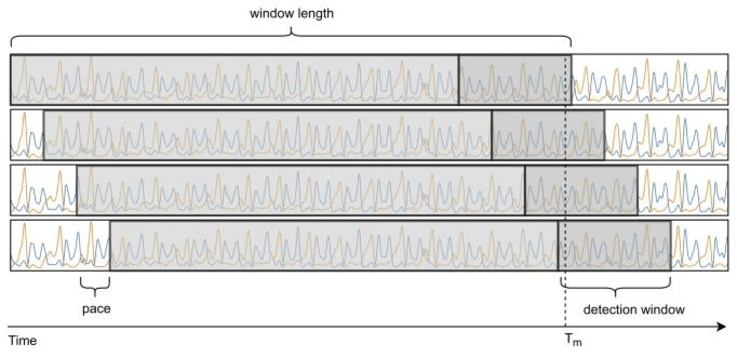
\includegraphics[width=\textwidth]{images/audio-nlp/waveform-segment.png}
        \caption*{Waveform segmented into overlapping frames and windowed (source: ResearchGate)}
    \end{figure}

    \framebreak

    \textbf{Summary of Pre‑processing Steps}
    \begin{enumerate}
        \item \textbf{Pre‑emphasis:} Boosts high frequencies.
        \item \textbf{Framing:} Splits signal into short, overlapping segments.
        \item \textbf{Windowing:} Applies Hamming window to each frame.
    \end{enumerate}
\end{frame}